\section{Детектирование нахождения в опасной зоне}
\begin{frame}
    \frametitle{Простейшее определение опасной зоны}
    В простейшем случае, опасную зону можно определить следующим образом.

    Зафиксируем выпуклый многоугольник $A$ на изображении.
    $$ x_{min} = \min\{ x : \exists y (x, y) \in A\} $$
    $$ x_{max} = \max\{ x : \exists y (x, y) \in A\} $$

    Тогда опасной зоной $DZ$ будем называть выпуклую оболочку множества
    $$ A \cup \{(x_{min}, 0), (x_{max}, 0)\} $$
\end{frame}

\begin{frame}
    \frametitle{Определение принадлежности опасной зоне}
    Задан минимальный порог срабатывания $m$ для принадлежности ключевой точки зоне.

    По определению $I_i = 1$, если ключевая точка человека $\left(x_i, y_i, c_i\right)$ находится в опасной зоне.
    $$ I_i = 1 \iff \left(c_i \ge m\right) \wedge \left(\left(x_i, y_i\right) \in DZ\right) $$

    Задана минимальная доля $t$ ключевых точек, принадлежащих опасной зоне, при которой считаем человека находящимся в ней.

    Считаем, что человек находится в опасной зоне, если:
    $$ \frac{\sum I_i}{N} \ge t $$
\end{frame}

\begin{frame}
    \frametitle{Усложнение определения опасной зоны}
    Будем считать, что область пространства, обозреваемого камерой, локально представляет из себя $\mathbb{R}^3$.

    Зафиксируем правильный многоугольник $A$ в плоскости $z = 0$.
    Тогда опасной зоной будем называть множество:
    $$DZ = \{(x, y, z) : (x, y, 0) \in A\} $$
\end{frame}

\begin{frame}
    \frametitle{Детектирование нахождения в опасной зоне}
    \begin{figure}
        \centering
        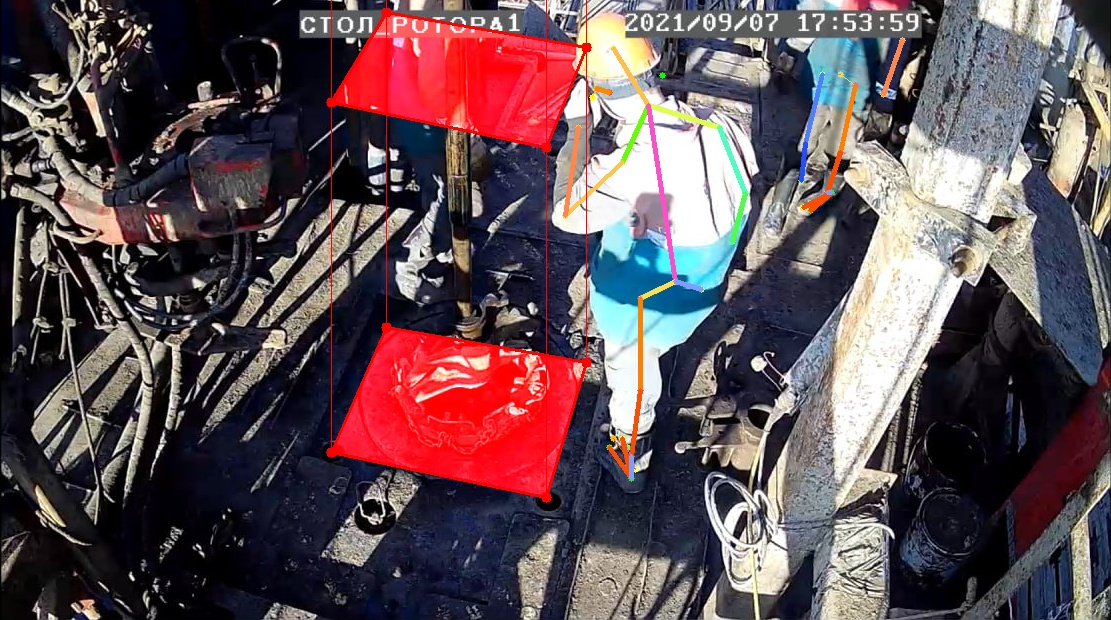
\includegraphics[width=1.0\textwidth,keepaspectratio]{danger_zone}
    \end{figure}
\end{frame}

\begin{frame}
    \frametitle{Усложнение определения опасной зоны}
    Перейдём от координат в $\mathbb{R}^3$ к обобщённым координатам в $\mathbb{P}^3$. Рассмотрим изображение как проективную плоскость $\mathbb{P}^2$ и найдём отображение $P_{3\times4}$:
    \begin{equation*}
        \left(
        \begin{array}{c}
            x \\
            y \\
            w
        \end{array}
        \right) =
        P_{3\times4}
        \left(
        \begin{array}{c}
            X \\
            Y \\
            Z \\
            T
        \end{array}
        \right)
    \end{equation*}

    Имея матрицу камеры $P_{3\times4}$ можно проверять что ключевые точки скелетной модели находятся внутри призмы представляющей собой опасную зону.
\end{frame}

\begin{frame}
    \frametitle{Пример центральной проекции}
    \begin{figure}
        \centering
        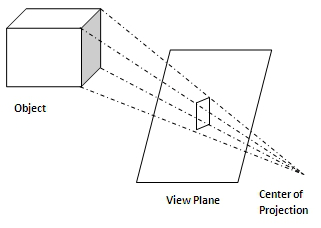
\includegraphics[width=1.0\textwidth,keepaspectratio]{central_projection}
    \end{figure}
\end{frame}